In addition to computing direct structural losses, OpenQuake also provides support for computing losses incurred for the following other loss types:

\begin{itemize}
\item{Non-structural losses}
\item{Contents losses}
\item{Downtime, or business interruption losses}
\item{Occupant fatalities}
\end{itemize}

The purpose of this case is to test the calculation of loss curves for the non-structural components for an asset. The replacement value of the non-structural components for the asset used in this case is $15,000$. Table~\ref{tab:vf-ln-tax1-nst} shows the mean loss ratios and corresponding coefficients of variation in the non-structural components vulnerability function used in this test case. Apart from the change in the vulnerability function and value, the calculation procedure remains the same as described in Case~1d.

The loss curve calculated using the implementation of the calculator in Julia is compared with that produced by OpenQuake in Figure~\ref{fig:lc-ebr-2a}.

\begin{figure}[htbp]
\centering
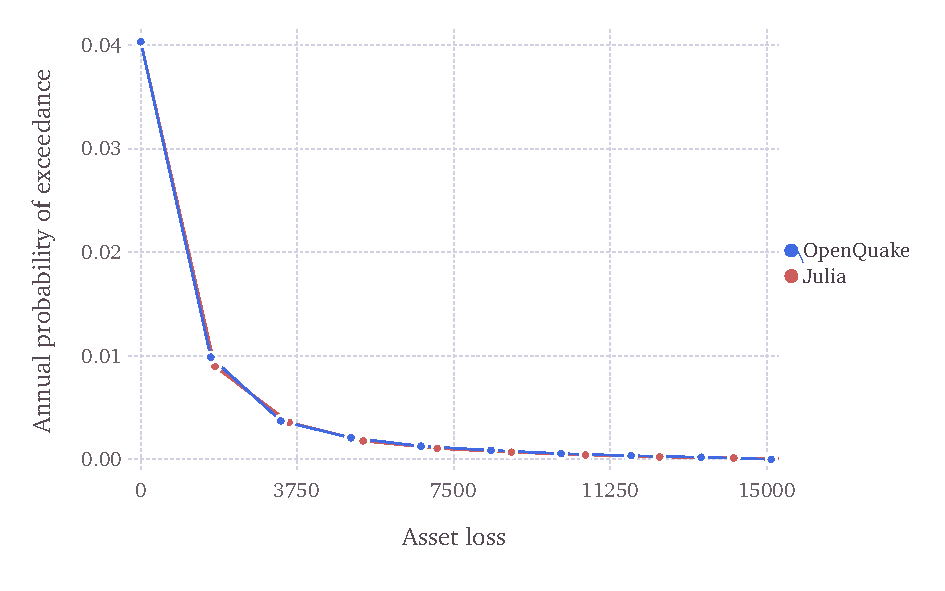
\includegraphics[width=12cm]{qareport/figures/fig-lc-ebr-2a}
\caption{Loss curve comparison for event based risk test case 2a}
\label{fig:lc-ebr-2a}
\end{figure}